\section{Ablation Study and Limitations}
\subsection{Ablation Study}
Table~\ref{tab:ablation} and Fig.~\ref{fig:ablation} show the ablation results. Removing ANN prediction increases delay and p95 delay. Removing cache value removes useful cache hit ratio and increases energy. Removing mobility-aware dwell gives lower average delay in this specific table, but it increases handovers sharply to 24.02 per 100 active cluster-slots. Removing neighbor cache almost halves the useful cache hit ratio. These results support the use of prediction, useful cache value, and dwell control as practical components of \pchorch.

\begin{table*}[!t]
\centering
\caption{Ablation results under combined stress. Energy is in kJ and ratio metrics are in percent.}
\label{tab:ablation}
\scriptsize
\begin{tabular}{lcccccccc}
\toprule
Variant & Avg Delay & p95 Delay & Energy & Handovers & Useful Cache & Outage & Drop & Throughput \\
\midrule
P3C-LR Core & 6.26 & 7.94 & 16.87 & 2.99 & 28.16 & 0.88 & 38.18 & 647.3 \\
No ANN prediction & 6.33 & 8.12 & 16.78 & 3.65 & 27.51 & 0.91 & 37.87 & 649.3 \\
No cache value & 6.46 & 8.12 & 20.21 & 3.35 & 0.00 & 0.79 & 38.39 & 645.4 \\
No mobility-aware dwell & 6.18 & 8.02 & 16.65 & 24.02 & 27.69 & 0.67 & 38.17 & 649.3 \\
No link-risk calibration & 6.28 & 8.14 & 16.64 & 2.95 & 28.47 & 0.96 & 38.03 & 644.3 \\
No neighbor cache & 6.29 & 7.94 & 17.28 & 3.09 & 14.21 & 0.90 & 38.52 & 643.3 \\
P3C-SR & 6.29 & 7.97 & 16.94 & 2.71 & 28.21 & 0.81 & 37.88 & 651.6 \\
ET-P3C & 6.26 & 7.91 & 16.93 & 2.60 & 27.80 & 0.91 & 38.14 & 647.1 \\
\bottomrule
\end{tabular}
\end{table*}


\begin{figure}[!t]
\centering
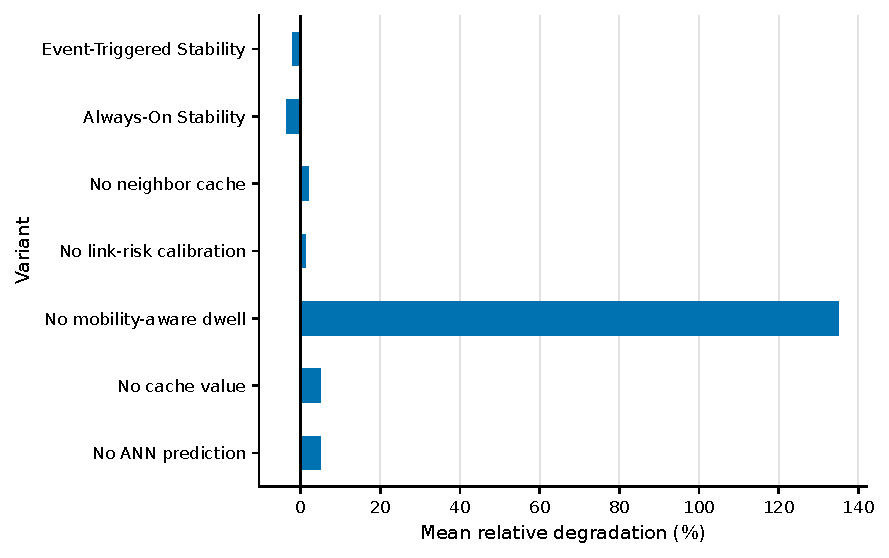
\includegraphics[width=\columnwidth]{figs/ablation_paperlock.pdf}
\caption{Ablation results for \pchorch. The figure shows the effect of removing prediction, cache value, dwell control, risk calibration, and neighbor cache reuse.}
\label{fig:ablation}
\end{figure}

\subsection{Stability Branch Analysis}
Fig.~\ref{fig:stability_branch} summarizes the stability branch. \psr\ is the stability-regularized internal variant and has the best aggregate non-oracle objective. However, earlier stability-focused branches did not give a clean, statistically reliable stability claim across all metrics. \etp\ is therefore reported as an exploratory ablation. This is why the paper is positioned as predictive 3C orchestration under link uncertainty, not as a pure stability-aware paper.

\begin{figure}[!t]
\centering
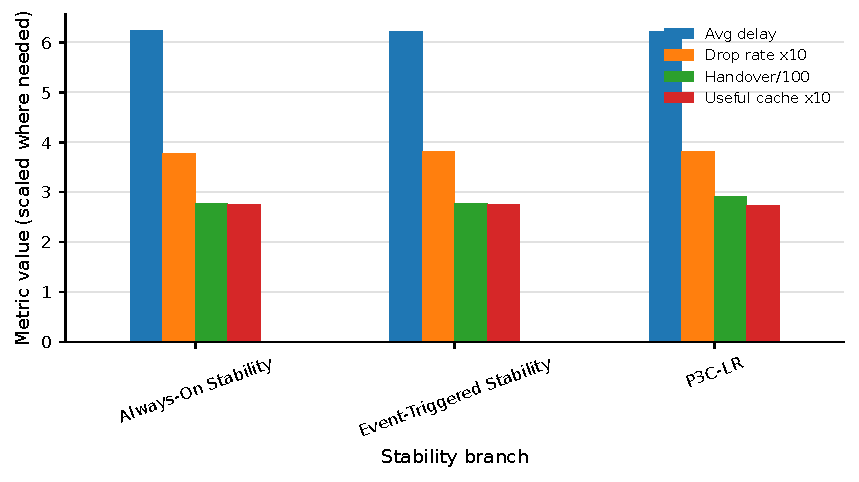
\includegraphics[width=\columnwidth]{figs/stability_negative_result_paperlock.pdf}
\caption{Stability branch analysis. \psr\ gives the best aggregate non-oracle objective, while \etp\ remains an exploratory ablation without a clear reliable gain over the simpler core.}
\label{fig:stability_branch}
\end{figure}

\subsection{Limitations}
This work has several limitations. First, the validation is simulation-based. Real UAV tests are needed before deployment. Second, the ANN predictor is trained on generated link data rather than real UAV field traces. Third, the weather model uses simplified clear, rainy, and rain-hot states. Fourth, security and privacy are not considered. Fifth, inter-UAV interference and detailed physical-layer beamforming are simplified. Sixth, \pclr\ does not improve every metric; it has a small energy cost and slightly lower useful cache hit ratio and drop-rate performance in some comparisons. Seventh, \etp\ did not provide reliable gain. Finally, real deployment will need hardware tests, controller delay measurement, and communication-delay validation.

These limitations do not remove the main result, but they define the next steps. Future work should use real link traces, online learning, interference-aware modelling, energy harvesting, and secure orchestration.
